\section{Methodology}

\begin{figure*}[!t]
    \centering
    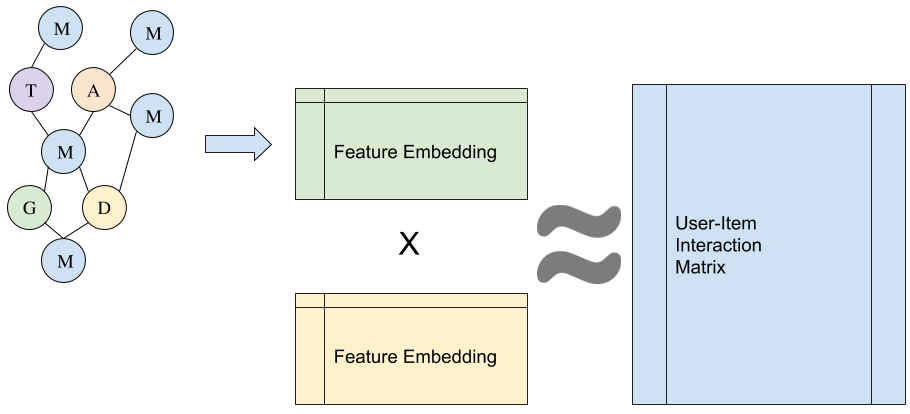
\includegraphics[width=0.8\textwidth]{figs/fig0.png}
    \caption{Overview}\label{fig:fe-overview}
\end{figure*}

In this Section, we propose a framework MERec (meta-path embedding based Recommendation) that allow recommendation models to learn item features embedding by adapting custom domain knowledge in a generic way. 

The key idea of our approaches is inspired by recent research on graph-based embedding \cite{dong2017metapath2vec}. Unlike traditional matrix based approach, learning user/item latent representation jointly based on user-item interactions matrix. Our approach breaks down item and user latent matrix learning through 2 separate steps. as illustrated in Fig \ref{fig:fe-overview}. Item embedding is first learned based on item and its features nodes within HIN with a user defined meta-path sets for the moderating its random walk process. Then user latent feature is trained though Factorization Machine, which is optimized by using Bayesian Probability Ranking.

\subsection{Learning Item presentation via Meta-path Based Random Walk}\label{3MF}

For items such as movies, books, music, there are a number of factors impacting users' decision. Instead of taking the one-hot encoding approach for category value. We first propose to treat different categorical information as separate node types. 
By leveraging domain knowledge we can form a heterogeneous information graph and sets of user defined meta-path for item-item similarities learning. 


\begin{figure*}[!t]
    \centering
    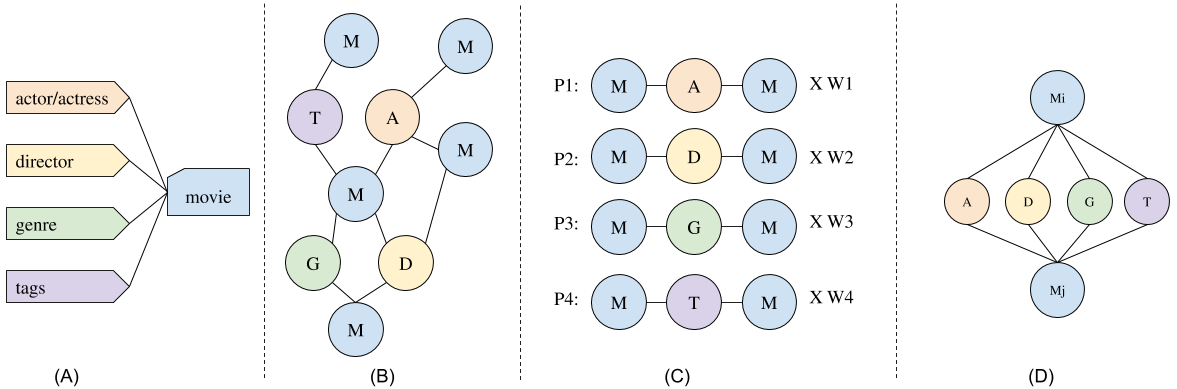
\includegraphics[width=0.8\textwidth]{figs/fig1.png}
    \caption{heterogeneous information graph based on item features}\label{fig:fe-graph}
\end{figure*}

For example, movie choice is closely linked to directors and its casts. Thus $Movie \rightarrow Director \leftarrow Movie$, $Movie \rightarrow Actor/Actress \leftarrow Movie$  can be very important meta-path in deciding how similar 2 movies are. We use those insights as a guideline to from a heterogeneous information graph based on item features. As shown in Fig \ref{fig:fe-graph}.
Each meta-path can derive a item-item similarity matrix $\mathbb{R}_i(\mathcal{P}_i)$, each different meta-path can be regarded as bias toward different feature aspects, so items co-occurrence can be learned separately under different meta-path.

as a result, item-item similarity score can be calculated by normalized meta-path similarity times meta-path weight.
\begin{equation}\label{itemsim}
    \mathcal{S}(v_i,v_j) = 
    \begin{cases}
         \sum\limits_{\substack{n=1}}^{n} \mathcal{R}_ij(\mathcal{P}_n,{W_n}),& \text{if } (v_{i}, .., v_{j}) \in \mathcal{P} \\
         0,              & \text{otherwise}
     \end{cases}
\end{equation}

$\mathcal{S}(v_i,v_j)$ stands for similarity between items $v_i$ and $v_j$ which shares the same node type. $R_ij()$ is a similarity function, where $\mathcal{P}_n, {W_n}$ stands for individual meta-path and its weights respectively. This end result provides guidance for the random walkers on our heterogeneous graph of item features. $(v_{i}, .., v_{j})$ is denoted as a meta-path instance, where $v_i$ is the starting node and $v_j$ the end node.

Given a heterogeneous graph $G = (V,E)$, and a meta-path set $[\mathcal{P}_1, \mathcal{P}_2, ... \mathcal{P}_n]$, the probability of transition is defined as following:

\begin{equation}\label{hetewalker}
    P(v_{i+1},\mathcal{P},w)= 
        \begin{cases}
            p({N^{t+1}(v_{i}^t)}),& \text{if } (v_{i+1}, .., v_{i}^t) \in \mathcal{P} \\
            0,              & \text{otherwise}
        \end{cases}
\end{equation}

$t$ is denoted as $t^th$ steps, as the walker traversing through the graph.
$p({N^{t+1}(v_{i}^t)})$ is a $softmax$ function on top of the neighbors of node $v_{i}^t$. 
that is:

\begin{equation}\label{softmaxwalker}
    p({N^{t+1}(v_{i}^t)}) = \frac{Exp(\mathcal{S}(v_i,v_j))}{\sum\limits_{\substack{n=1}}^{n} {Exp(\mathcal{S}(v_i,v_j)})}
\end{equation}

we enable skip-gram to learn the presentation of given node $v$:

\begin{equation}\label{skipgram}
    arg max
    \sum\limits_{\substack{v \in V}}
    \sum\limits_{\substack{c \in N(v)}}
    log p({c|v;\theta})
\end{equation}

$log p({c|v;\theta}))$ is the softmax function as defined in \cite{mikolov2013distributed} \cite{mikolov2013efficient}. In our approach, we substitute $log p({c|v;\theta}))$ with softmax function defined in equation \ref{softmaxwalker}. $c$ is denoted as $context$, in graph structure setting, $c$ is the neighboring nodes of given node $v$, i.e. $N(v)$. 

During the item embedding learning, we introduce 3 hyper parameters to learn the item vector representation. $d$ for dimension size, $x$ for number of walks, and $l$ for depth of each random walk.

\subsection{User latent feature learning based on item embedding}\label{3PCC}

In order to solve pure cold start problem, commonly feature based (content based) are one of limited way to make recommendation. 
Additionally, we adopt Pearson Correlation Coefficient (PCC) to be in combination with MERec through the recommendation process. 
PCC is a popular measurement approach as defined in equation \ref{pcc}, unlike Cosine Similarity, PCC takes the difference of mean and variance between users' rating scale into account.


    \begin{equation}\label{pcc}
        S_{u_i,u_j}^{PCC} = 
        \dfrac{
            \sum_{v \in V_{u_i} \cap V_{u_j}} (r_{u_i,v}-\overline{r_{u_i}}) 
            * 
            (r_{u_j,v} - \overline{r_{u_j}})
        }
        {
            \sqrt{\sum_{v \in V_{u_i} \cap V_{u_j}} (r_{u_i,v}-\overline{r_{u_i}})^2} 
            * 
            \sqrt{\sum_{v \in V_{u_i} \cap V_{u_j}} (r_{u_j,v}-\overline{r_{u_j}})^2}
        }
    \end{equation}

accordingly, we can normalized the user-item rating based on normalized user rating $\overline{u}$ overall:
\begin{equation}\label{pcc}
    NS(r_{u_i,v_j}) =  S_{u_i,\overline{u}}^{PCC}
\end{equation}

Consequently, we get the top ranked user by calculating as following:

% \begin{algorithm}
%     \caption{ranked users list}
%     \begin{algorithmic}[1] 
%     \REQUIRE~~\\ %Input
%     New Item: $v$\\
%     Existing user item ratings: ${R_{mxn}}$\\
%     Items vectors: $\mathcal{V}$\\
%     Top X nearest items: $X$\\
%     Top K ranked users list rank: $K$\\
%     \ENSURE~~\\ %Output
%     \STATE Compute nearest items $TopN(v,\mathcal{V})$ based on $\mathcal{V}$ and $v$
%     \STATE \textbf{for} x=1 : X
%     \STATE \quad Compute normalized rating per user of $v_x$
%     \STATE \quad Ranked users $RankedList(v_x) \leftarrow (u_i, NS(r_{u_i,v_x}))$
%     \STATE \quad $TopKList(v) \leftarrow$ Top $K$ (user,rating) in $RankedList(v_x)$
%     \STATE $RankedList(v)$ = \textbf{from} $TopKList(v)$ \textbf{group by} user \textbf{select} (user,$\sum{rating}$) \textbf{order by} $\sum{rating}$
%     \RETURN Top K of $RankedList(v)$
%     \end{algorithmic}\label{alg:1}
% \end{algorithm}

In Section \ref{4_experiment}, we would show more detailed comparison results with traditional categorical one-hot encoding approach

\subsection{Sparse Recommendation: MERec-BPR}\label{3BPR}
One of the other common cold start problem, that we commonly facing is sparse data. Matrix Factorization or CF based approach, try to learn user and item presentation (i.e. $U, V$) in a latent space jointly, normally suffers from data sparsity problem.


Here we propose, instead of learning $U, V$ jointly, we replace $V$ with meta-path based vectors $Vec(v)$. This approach provides several benefits:
\begin{enumerate}
        \item Reducing learning complexities
        \item Taking both item features and user-item interactions into account
        \item $Vec(v)$ is less impacted when user-item interactions are sparse 
\end{enumerate}

We use BPR as our optimization objective:

\begin{equation}\label{skipgram}
    arg max (u_i \cdot Vec(v)-u_j \cdot Vec(v)) - \dfrac{\lambda}{2}tr(U^TU)
\end{equation}


Based on the experiment result in Section \ref{4_experiment}, we see MERec out performs widely used CF+ BPR by a large margin in sparse dataset. It also gained equivalent or minor advantage when the dataset is less sparse in non-cold start settings.


